% The eventually consistent page: tiered pagination for live LuaLaTeX editing
% TUGboat article draft.
\documentclass{ltugboat}
\usepackage{microtype}
\usepackage{graphicx}
\usepackage{booktabs}
\usepackage{tikz}
\usetikzlibrary{arrows.meta, positioning, shapes.geometric}
\usepackage[hidelinks,pdfa]{hyperref}

\def\LuaTeX{Lua\TeX}
\def\LuaLaTeX{Lua\LaTeX}
\setlength{\emergencystretch}{1.5em}

\title{The eventually consistent page:\\ tiered pagination for live
\LuaLaTeX{} editing}
\author{Srikanth Mohankumar}
\address{TNQ Tech, Chennai, India}
\netaddress{srikanth.mohan (at) tnqtech dot com}

\begin{document}
\maketitle

\begin{abstract}
Recent work has shown that a single paragraph of a \LuaLaTeX{} document can
be re-typeset in about a millisecond inside a persistent engine, because
Knuth--Plass line breaking depends only on the paragraph and a finite
parameter context. We report on carrying that observation into journal
production: a system in which every keystroke is routed by its
\emph{pagination impact}. Edits that provably cannot move anything else on
any page patch a cached page description in place, with no compilation at
all; edits that change a paragraph's height reflow the column approximately
on screen while a warm, preamble-resident engine re-typesets the document
body in about three seconds; and the true PDF follows a few seconds later.
Pages are thus \emph{eventually consistent}, in the database sense: the
paragraph under the cursor is always exact, and every other page converges
to ground truth shortly after. We describe the context capture needed for
scaled-point-exact isolated recompilation, the tier tests, the single-shot
warm-engine pool that survived a real production template, and measurements
on live journal articles with structure tagging and data-driven float
placement.
\end{abstract}

\section{A production problem}

A typesetting house compiles \LaTeX{} continuously: manuscripts arrive,
are normalized into a house markup, composed, corrected, and recomposed,
often dozens of times per article. Each correction cycle today costs a full
compilation. On the production article used throughout this paper---a
ten-page, two-column chemistry journal article with structure tagging,
OpenType fonts, and data-driven float placement---one compilation takes
about eighteen seconds, of which the template preamble alone accounts for
thirteen. An operator who moves a comma waits as long as one who rewrites
a section.

Lode's recent measurement~\cite{lode:realtime} reframed the problem: the
line breaker itself needs only fractions of a millisecond per paragraph,
so the latency of the edit loop is architectural, not algorithmic. His
\textsf{texlode} editor demonstrated per-paragraph recompilation with a
background full compile for global layout. Earlier systems attacked the
same latency from other directions: \TeX presso resumes a modified \XeTeX{}
from fork-based snapshots~\cite{texpresso}, and Typst rebuilt the engine
around memoized incremental evaluation~\cite{haug:thesis}, which is fast
but reconverges the whole layout on every edit and does not read \LaTeX.

This paper describes an independent implementation of the
paragraph-local idea, taken further in three directions that production
imposed on us. First, \emph{exactness}: an isolated recompilation must
reproduce the reference document to the scaled point, under full
\textsf{microtype}, custom fonts, and a heavyweight commercial template.
Second, \emph{pagination-impact routing}: most keystrokes need no
repagination at all, and the system should know that. Third,
\emph{engine economics}: when the preamble costs thirteen seconds, neither
paying it per edit nor trusting a long-lived engine's state is acceptable;
we ended up with disposable warm engines.

\section{The locality dividend}

Knuth--Plass line breaking is a pure function: given the horizontal list of
a paragraph and a finite set of parameters, it returns the same line boxes
regardless of what precedes or follows the paragraph in the
document~\cite{knuthplass}. \LuaTeX{} makes both sides of this function
observable. Callbacks around the line breaker
(\verb|pre_linebreak_filter|, \verb|post_linebreak_filter|) expose the
horizontal list and the resulting lines; the \verb|node| library lets Lua
walk those lines and measure every glyph position with the engine's own
arithmetic.

The dividend is that a document decomposes into two regimes. Line breaking
is $O(\hbox{paragraph})$ and embarrassingly local; page breaking, float
placement, marks, and cross-references are global and stateful. A live
editor can therefore keep the local regime synchronous---inside the
16\,ms budget of a display frame---and make the global regime
\emph{eventually consistent}: always converging, never blocking.

\section{Architecture}

\begin{figure*}[t]
\centering
% Figure 1 — system architecture (wide, two-column span)
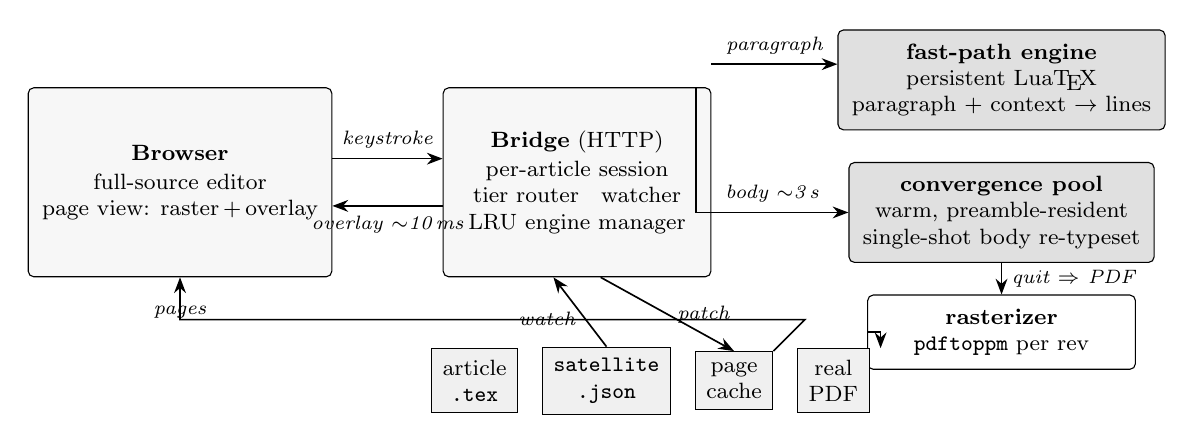
\begin{tikzpicture}[
  font=\footnotesize,
  box/.style={draw, rounded corners=2pt, align=center, inner sep=5pt,
              minimum height=8mm},
  store/.style={draw, align=center, inner sep=4pt, fill=black!6},
  eng/.style={box, fill=black!12},
  lbl/.style={font=\scriptsize\itshape, midway},
  arr/.style={-{Stealth[length=2mm]}, semithick},
  node distance=6mm and 10mm]

  % client
  \node[box, fill=black!3, minimum width=30mm, minimum height=24mm]
    (browser) {\textbf{Browser}\\[1pt]
      full-source editor\\ page view: raster\,+\,overlay};

  % bridge
  \node[box, fill=black!3, minimum width=34mm, minimum height=24mm,
        right=14mm of browser]
    (bridge) {\textbf{Bridge} (HTTP)\\[1pt]
      per-article session\\ tier router \; watcher\\ LRU engine manager};

  % engines column
  \node[eng, right=16mm of bridge, yshift=13mm, minimum width=34mm]
    (fast) {\textbf{fast-path engine}\\ persistent \LuaTeX\\
            paragraph + context $\to$ lines};
  \node[eng, below=4mm of fast, minimum width=34mm]
    (pool) {\textbf{convergence pool}\\ warm, preamble-resident\\
            single-shot body re-typeset};
  \node[box, below=4mm of pool, minimum width=34mm]
    (raster) {\textbf{rasterizer}\\ \texttt{pdftoppm} per rev};

  % stores under bridge
  \node[store, below=9mm of bridge, xshift=-13mm] (tex) {article\\ \texttt{.tex}};
  \node[store, right=3mm of tex] (sat) {\texttt{satellite}\\ \texttt{.json}};
  \node[store, right=3mm of sat] (cache) {page\\ cache};
  \node[store, right=3mm of cache] (pdf) {real\\ PDF};

  % flows
  \draw[arr] ([yshift=3mm]browser.east) -- ([yshift=3mm]bridge.west)
    node[lbl, above] {keystroke};
  \draw[arr] ([yshift=-3mm]bridge.west) -- ([yshift=-3mm]browser.east)
    node[lbl, below] {overlay $\sim$10\,ms};
  \draw[arr] (bridge.east|-fast.west) ++(0,2mm) -- ([yshift=2mm]fast.west)
    node[lbl, above] {paragraph};
  \draw[arr] (bridge.north east) ++(-2mm,0) |- (pool.west)
    node[lbl, above, pos=.75] {body $\sim$3\,s};
  \draw[arr] (pool.south) -- (raster.north)
    node[lbl, right] {quit $\Rightarrow$ PDF};
  \draw[arr] (raster.west) -| ([xshift=6mm]pdf.north);
  \draw[arr] (sat.north) -- ([xshift=-3mm]bridge.south)
    node[lbl, left, pos=.4] {watch};
  \draw[arr] (bridge.south) ++(3mm,0) -- (cache.north)
    node[lbl, right, pos=.5] {patch};
  \draw[arr] (cache.north east) -- ++(4mm,4mm) -| (browser.south)
    node[lbl, below, pos=.78] {pages};
\end{tikzpicture}

\caption{System overview. A browser edits the full source; a small bridge
routes each edit to the cheapest sufficient mechanism. The fast-path
engine is a persistent \LuaLaTeX{} that re-breaks single paragraphs; the
convergence pool holds warm, preamble-resident engines that re-typeset the
document body once each and then finalize a real PDF{}.}
\label{fig:arch}
\end{figure*}

Figure~\ref{fig:arch} shows the pieces. Paragraphs in our production
markup are wrapped
\begin{center}\small
\verb|\tagStructPara{}\paraid{para10}|\,\dots\\
\verb|...\tagStructParaEnd{}|
\end{center}
so paragraph identity already exists in the
source; the same \verb|\paraid| plants a node attribute during an
instrumented reference compilation, keying three artifacts to each
paragraph: its \emph{context} (below), a \emph{reference signature} (the
width, height, depth, and exact glyph positions of every line), and its
location in a \emph{page cache}---the absolute display list of every
shipped page, captured in a \verb|pre_shipout_filter| walk.

\subsection{Exact isolated recompilation}

A paragraph is re-typeset in a persistent engine that loaded the article's
own preamble once. The request wraps the paragraph source in a
\verb|\vbox| preceded by a prologue that reinstates the captured context:
the measure and shape (\verb|\hsize|, \verb|\parshape|,
\verb|\hangindent|), the font in force at paragraph start, the hyphenation
language and limits, tolerance and emergency stretch, penalties and
demerits, interword and interline spacing
(\verb|\baselineskip|, \verb|\lineskip|, \verb|\lineskiplimit|), and the
\textsf{microtype} switches---about twenty-five parameters in all.
Cross-reference state is transplanted by defining \verb|\r@|\dots{} and
\verb|\b@|\dots{} macros directly from the reference \verb|.aux| via
\verb|token.set_macro| (the \LaTeX{} kernel refuses
\verb|\newlabel| mid-document).

Three details decide between ``close'' and ``exact.''
\emph{Engine arithmetic}: glyph advances must be measured with
\verb|node.dimensions|, whose C~implementation folds in
\textsf{microtype} font expansion and expanded font kerns; summing
\verb|glyph.width| by hand is wrong by several points per justified line.
\emph{The start font}: \verb|pre_linebreak_filter| sees the font at
paragraph \emph{end}; the font at paragraph \emph{start} must be captured
in \verb|insert_local_par|.
\emph{Leading glue}: the reference lines carry the interline glue computed
against the \emph{previous} paragraph's depth, which an isolated
\verb|\vbox| cannot reproduce, so all comparisons are made relative to the
first baseline. With these in place, re-typesetting an unchanged paragraph
of the production article reproduces every glyph position to zero scaled
points, and does so in about ten milliseconds per request.

\subsection{Tier 0: edits that cannot repaginate}

\begin{figure}[tb]
\centering
% Figure 2 — tier routing of an edit (column width)
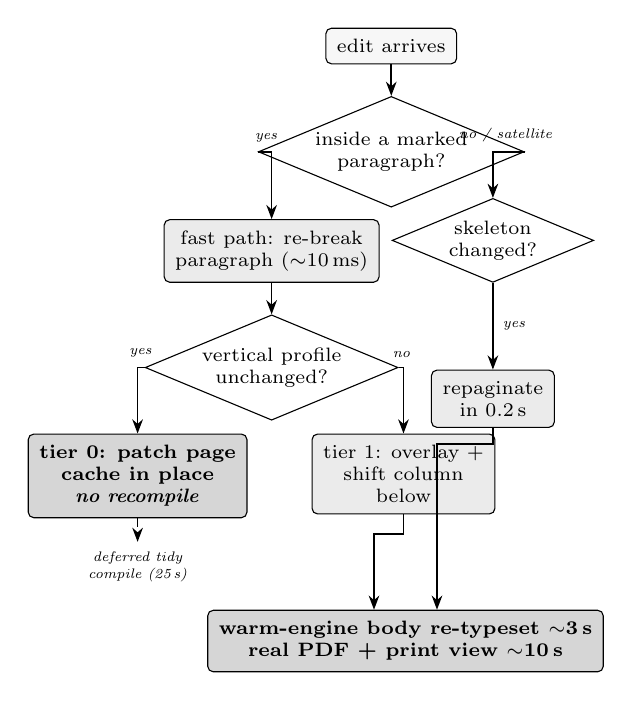
\begin{tikzpicture}[
  font=\footnotesize,
  q/.style={draw, diamond, aspect=2.4, align=center, inner sep=1pt,
            font=\scriptsize},
  act/.style={draw, rounded corners=2pt, align=center, inner sep=4pt,
              fill=black!8, font=\scriptsize},
  fin/.style={draw, rounded corners=2pt, align=center, inner sep=4pt,
              fill=black!16, font=\scriptsize\bfseries},
  arr/.style={-{Stealth[length=1.8mm]}, semithick},
  lb/.style={font=\tiny\itshape},
  node distance=4mm and 3mm]

  \node[act, fill=black!3] (edit) {edit arrives};
  \node[q, below=of edit] (inpara) {inside a marked\\ paragraph?};
  \node[act, below left=5mm and -7mm of inpara] (fastpath)
    {fast path: re-break\\ paragraph ($\sim$10\,ms)};
  \node[q, below=of fastpath] (profile) {vertical profile\\ unchanged?};
  \node[fin, below left=5mm and -5mm of profile] (patch)
    {tier 0: patch page\\ cache in place\\ \emph{no recompile}};
  \node[act, below right=5mm and -3mm of profile] (shift)
    {tier 1: overlay +\\ shift column\\ below};
  \node[q, below right=5mm and -8mm of inpara, xshift=6mm] (struct)
    {skeleton\\ changed?};
  \node[act, below=11mm of struct] (now) {repaginate\\ in 0.2\,s};
  \node[fin, below=24mm of profile, xshift=17mm] (conv)
    {warm-engine body re-typeset $\sim$3\,s\\
     real PDF + print view $\sim$10\,s};

  \draw[arr] (edit) -- (inpara);
  \draw[arr] (inpara) -| node[lb, above, pos=.3] {yes} (fastpath);
  \draw[arr] (inpara) -| node[lb, above, pos=.3] {no / satellite} (struct);
  \draw[arr] (fastpath) -- (profile);
  \draw[arr] (profile) -| node[lb, above, pos=.3] {yes} (patch);
  \draw[arr] (profile) -| node[lb, above, pos=.3] {no} (shift);
  \draw[arr] (struct) -- node[lb, right] {yes} (now);
  \draw[arr] (shift.south) -- ++(0,-2.5mm) -| ([xshift=-4mm]conv.north);
  \draw[arr] (now.south) -- ++(0,-2mm) -| ([xshift=4mm]conv.north);
  \draw[arr, dashed] (patch.south) -- ++(0,-3mm)
    node[lb, below, align=center] {deferred tidy\\ compile (25\,s)};
\end{tikzpicture}

\caption{Routing an edit by its pagination impact.}
\label{fig:tiers}
\end{figure}

Define a paragraph's \emph{vertical profile} as the sequence
$(y_i - y_1, h_i, d_i)$ over its lines: baseline offsets relative to the
first baseline, plus each line's height and depth. If an edit leaves the
profile identical, the paragraph occupies exactly the same vertical
extent, so \emph{nothing else on any page can move}. The bridge then
patches the paragraph's glyphs directly into the page cache---about
thirty milliseconds end to end, with no engine run beyond the fast path
itself---and defers any compilation to an idle tidy pass
(figure~\ref{fig:tiers}).

The profile test is exact, and honestly so: replacing
\emph{software} by \emph{programs} in one test paragraph was routed to
repagination because the descenders of \emph{p} and \emph{g} deepen the
last line by 0.18\,pt, which really does shift everything below it. In
practice most keystrokes---replacing words of similar metrics, fixing
punctuation, editing within a line---are tier~0.

\subsection{Tier 1: approximate now, exact shortly}

When the profile changes, the browser immediately shifts the same-column
material below the edited paragraph by the height difference, word-processor
style, while a real repagination runs. Deleted paragraphs likewise vanish
from the page at the keystroke. These client-side motions are approximate
(they do not re-cut page boundaries); they exist to keep the page
perceptually continuous for the two or three seconds the truth takes.

Edits outside any marked paragraph---headings, floats, preamble---and
changes to supporting data files are detected by diffing a \emph{skeleton}
of the source (paragraph bodies blanked) and routed to immediate
repagination.

\subsection{Warm, single-shot convergence engines}

\begin{figure}[tb]
\centering
\resizebox{\columnwidth}{!}{% Figure 3 — warm single-shot engine lifecycle (column width)
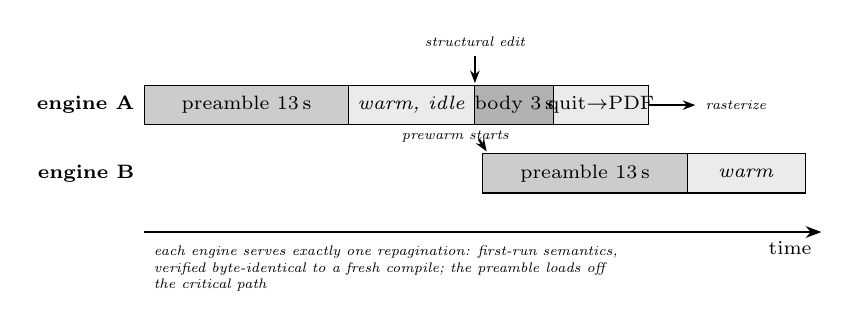
\begin{tikzpicture}[font=\scriptsize, yscale=.62]
  % time axis
  \draw[-{Stealth[length=2mm]}] (0,0) -- (8.6,0) node[below left] {time};

  % engine A lane
  \node[left, font=\scriptsize\bfseries] at (0,2.6) {engine A};
  \draw[fill=black!20] (0,2.2) rectangle node{preamble 13\,s} (2.6,3.0);
  \draw[fill=black!8]  (2.6,2.2) rectangle node{\emph{warm, idle}} (4.2,3.0);
  \draw[fill=black!30] (4.2,2.2) rectangle node{body 3\,s} (5.2,3.0);
  \draw[fill=black!8]  (5.2,2.2) rectangle node{quit$\to$PDF} (6.4,3.0);

  % engine B lane (prewarm)
  \node[left, font=\scriptsize\bfseries] at (0,1.2) {engine B};
  \draw[fill=black!20] (4.3,0.8) rectangle node{preamble 13\,s} (6.9,1.6);
  \draw[fill=black!8]  (6.9,0.8) rectangle node{\emph{warm}} (8.4,1.6);

  % events
  \draw[-{Stealth[length=1.6mm]}, thick] (4.2,3.6) -- (4.2,3.05);
  \node[above, font=\tiny\itshape] at (4.2,3.6) {structural edit};
  \draw[-{Stealth[length=1.6mm]}, thick, dashed] (4.25,1.9) -- (4.35,1.65);
  \node[right, font=\tiny\itshape] at (3.15,1.95) {prewarm starts};
  \draw[-{Stealth[length=1.6mm]}, thick] (6.4,2.6) -- (7.0,2.6)
    node[right, font=\tiny\itshape] {rasterize};

  % annotation
  \node[align=left, font=\tiny\itshape, anchor=west] at (0, -0.75)
    {each engine serves exactly one repagination: first-run semantics,\\
     verified byte-identical to a fresh compile; the preamble loads off\\
     the critical path};
\end{tikzpicture}
}
\caption{Convergence engine lifecycle. Engines are used exactly once;
replacements pay the preamble in the background.}
\label{fig:engines}
\end{figure}

Repagination is a full re-typeset of the document body. Paying the
thirteen-second preamble each time would dominate; a preamble format dump
is not an option under \textsf{luaotfload} (we measured a 66\,MB format
that then failed to run); and reusing one long-lived engine for many body
passes failed \emph{validation}: our first design restored count and dimen
registers between runs, and run~one was byte-identical to a fresh
compile---but run~two lost the figure pages, because the template's float
machinery keeps global state the register snapshot does not cover.

The design that survived is shown in figure~\ref{fig:engines}: a pool of
\emph{single-shot} engines. Each has the preamble resident and serves
exactly one repagination---guaranteed first-run semantics, the case we
proved exact---then receives a graceful \verb|\end{document}| so the PDF
trailer is finalized, and a replacement warms up off the critical path.
The body re-typeset takes about three seconds on the production article;
consecutive structural edits are absorbed by the pool. One practical note:
after its answer is read, a quitting engine still writes end-of-document
chatter, and blocks forever if nobody drains the pipe. The PDF is
rasterized in the background and displayed as the page image, with live
overlays drawn above it; the on-screen page is the real page, typically
ten seconds after the edit that invalidated it.

\subsection{Supporting data, not just source}

Journal production changes more than the \verb|.tex|. In our pipeline a
\verb|satellite.json| drives float placement (anchor paragraphs, order,
dimensions). Because the template activates it \emph{after}
\verb|\maketitle|---at body time, not preamble time---every single-shot
engine reads the current file, so satellite edits repaginate correctly
with no engine restart; a file watcher makes them do so automatically,
in the same three seconds as a structural source edit.

\section{Measurements}

\begin{table}[tb]
\centering
\small
\begin{tabular}{@{}lr@{}}
\toprule
event & latency \\
\midrule
fast path, demo article (IEEE class) & 1--3\,ms \\
fast path, production article & $\sim$10\,ms \\
tier-0 in-place page patch & $\sim$30\,ms \\
repagination (warm engine, body only) & $\sim$3\,s \\
real PDF rasterized (print view) & $\sim$10\,s \\
\midrule
full compile of the same article & 18.2\,s \\
\quad of which template preamble & 13.1\,s \\
\bottomrule
\end{tabular}
\caption{The latency ladder on a ten-page production journal article
(LuaHB\TeX{} 1.22.0, \TeX{} Live 2025, commodity Linux).}
\label{tab:latency}
\end{table}

Fidelity was evaluated first on four public classes
(\textsf{elsarticle}, \textsf{IEEEtran}, \textsf{acmart},
Elsevier \textsf{cas-dc}): across twelve marked body paragraphs per class,
ten recompiled byte-exactly---zero scaled points of deviation in every
glyph position, with full \textsf{microtype}---and the two exceptions per
class are the principled ones, a footnote (insertions couple to the page
builder) and a display equation (partial-paragraph shapes). The same
harness then passed unchanged on the production article and on a second
article taken directly from the production queue, sixty-one paragraphs,
including a twenty-eight-line paragraph exact at 171\,ms.

Table~\ref{tab:latency} summarizes the latency ladder. The number we care
about most in production is the gap between rows: an operator's common
edits sit three orders of magnitude below the compile they used to pay,
and even the worst structural edit converges six times faster than a
fresh compile---entirely because the preamble no longer sits on the
critical path. (Profiling that preamble was a side benefit: over five
seconds of CPU inside one typesetting model configuration, and the same
mathematics font parsed twice from two paths.)

\section{Boundaries and future work}

The fast path refuses, correctly, what it cannot do exactly: paragraphs
with footnotes, displayed equations, or list labels take the repagination
path; the abstract, set inside the frontmatter machinery, is not
paragraph-editable. All of these still converge in seconds.

The open problem is sub-second repagination. Every paragraph's line boxes
are already cached; what remains global is cutting pages, and a
\emph{galley re-cut}---re-running only the page builder over cached lines
from the edited page onward---would bring structural edits near the frame
budget too. Floats, insertions, and marks make this a genuine project
rather than an optimization. Until then, the eventually consistent page
has proven a comfortable contract: the paragraph under your cursor is
always the truth, and the rest of the document is never more than a few
seconds behind it.

\SetBibJustification{\raggedright}
\begin{thebibliography}{9}
\bibitem{knuthplass} D.\,E. Knuth, M.\,F. Plass.
Breaking paragraphs into lines.
\emph{Software---Practice and Experience} 11(11):1119--1184, 1981.

\bibitem{lode:realtime} C. Lode.
Real-time \LuaTeX: recompiling large documents in 1\,ms.
TUG 2026 preprint, \url{tug.org/tug2026/preprints/lode-realtime.pdf}.

\bibitem{texpresso} F. Bour.
\TeX presso: live rendering and error reporting for \LaTeX.
\url{github.com/let-def/texpresso}.

\bibitem{haug:thesis} M. Haug.
Fast typesetting with incremental compilation.
Master's thesis, Technische Universit\"at Berlin, 2022.
\end{thebibliography}

\makesignature
\end{document}
